\subsection{Slicing based hypervisors}
\label{sec:existing-nhv}
In this section, we describe the hypervisors using the slicing technique to abstract the physical infrastructure into Virtual Networks.

\subsubsection{FlowVisor}

FlowVisor~\cite{FlowVisor-Sherwood2009} is the first SDN hypervisor ever implemented.
FlowVisor creates Virtual Networks by slicing the physical infrastructure, providing each tenant with a set of physical resources (\ie a slice).
The tenant will then assign a flowspace to each physical node he has been allocated.
The flowspace corresponds to the set of flow rules that are used as filters for the tenant's traffic.
Finally, the Virtual Network\GB{you used to capitalize the term ``Virtual Network''. Please be consistent throughout the manuscript} presented to the tenant is the set of physical nodes that match the incoming traffic defined by the allocated flowspace.
The tenant then connects their SDN controller to the slice, enabling them to interact with their Virtual Network.

% Virtual Networks are defined as a set of links between physical SDN switches.
% These links will only match the traffic belonging to the tenant.
% FlowVisor introduce them as flowspace and each flowspace maps a tenant with a physical node and a specific match-action criteria for the traffic.
% For a tenant, the collection of these flowspaces is called a slice and represent their Virtual Network. 


\begin{figure}[ht]
    \centering
    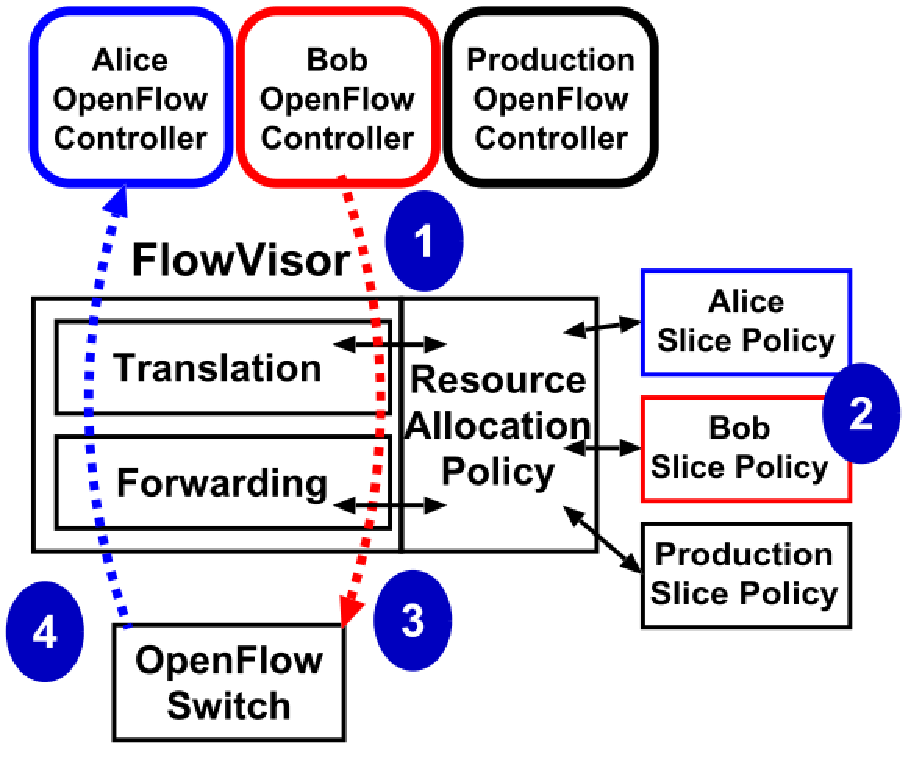
\includegraphics[scale=0.6]{figures/flowvisor-process.pdf}
    \caption{Message processing in Flowvisor~\cite{FlowVisor-Sherwood2009}}
    \label{fig:flowvisor-process}
\end{figure}

FlowVisor enforces isolation between tenants by acting as a proxy between them and the physical infrastructure, as depicted in Figure~\ref{fig:flowvisor-process}.
FlowVisor abstracts the physical architecture by showing each tenant only the resources that have been allocated to each of them.
When a tenant wants to deploy an OpenFlow rule (OF rule) on a physical node (1), FlowVisor intercepts it, checks the resources allocated to the slice (2) and rewrites match and action fields so the rule only affects the Virtual Network and not all the incoming traffic (3).
Similarly, when an OpenFlow message is sent from a physical node to the controller, FlowVisor intercepts the message and forwards it only to the tenants whose slice's policy matches the message (4).
Precisely, the flowspace assigned to the slice serves as an identifier to determine to which tenant the message should be forwarded.

Flowvisor provides mechanisms to enforce isolation mechanisms for the bandwidth, topology, switch CPU, flowspace, flow tables and the SouthBound Interface\GB{you used to capitalize the term ``SouthBound Interface''. Please stay consistent throughout the manuscript.} communications (\ie rewriting OF messages to prevent overlapping of identifiers used by controllers belonging to different tenants).
Bandwidth isolation is enforced by assigning flows to different QoS queues using the VLAN PCP field.
CPU isolation is done by either limiting the rate of tenant messages to switches, or by rewriting flow rules to limit the number of messages that would be generated by the switch.
Isolating these resources will prevent a tenant from exceeding the amount of resources he has been allocated or prevent a malicious or misconfigured flow rule from modifying the traffic of another user without authorization.
However, FlowVisor does not implement major components related to virtualization, such as arbitrary topologies and Virtual Network migration.
This can be explained because the slicing of physical resources makes it impossible for the hypervisor to define a new physical substrate that would be suited for the new embedding of the Virtual Network.
These aspects have been tackled in several subsequent hypervisors based on FlowVisor.

\subsubsection{Enhanced FlowVisor}
Enhanced FlowVisor~\cite{EnhancedFV-Min2012} extends FlowVisor by implementing an admission control process that verifies if a new Virtual Network request can be accepted in the infrastructure. 
Information about Virtual Networks, tenants information, among others, are stored in a database. When a new request for a Virtual Network is received, a potential physical substrate will be mapped to the request. Then Enhanced FlowVisor will query the database to check if each link in the physical substrate satisfies the requested bandwidth of the Virtual Network. If it cannot, then the request is denied. 
If it can, the flowspace is assigned an identifier based on 3 bits of the VLAN PCP field which restricts the total number of tenants to 8.
Enhanced FlowVisor includes a minimum guaranteed bandwidth feature. It ensures that each tenant of a Virtual Network will be served with the required amount of bandwidth for all the links in his topology.
Instead of using the VLAN PCP field to enforce bandwidth isolation, Enhanced FlowVisor uses a feature deployed in certain switches: the Guaranteed Minimum Bandwidth (GMB).
Enhanced FlowVisor is based on the NOX controller and uses HP ProCurve switches that implement the bandwidth isolation feature.

\subsubsection{Slices Isolator}
Slices Isolator~\cite{SlicesIsolator-El-Azzab2011} is an\GB{it seems to be ``a'' hypervisor rather than ``an'', according to Wikipedia. Please check the articles in your manuscript.} hypervisor providing resource isolation between slices. A slice is defined as a subdivision of the physical infrastructure, to which flows will be assigned. Slices Isolator provides isolation for interfaces, flow processing and memory. Interface isolation consists in either providing a dedicated network interface to a slice or to aggregate incoming traffic to one interface and then distributing the control to the different tenants. Processing isolation defines which flows will be processed using the same set of rules.
% \GB{not clear: is slicing done per flow entry or per flow table?}. 
% \GB{the following example's purpose is not very clear}
Each flow is divided into two subflows,  The first subflow is processed by the switch, and the other one is discarded. This can be illustrated by considering all traffic with destination port 80 (Web traffic) but only accepting traffic within a specific IP range (the customer's web server) and dropping the rest. This helps reducing the size of processing tables but if a poorly designed rule is added, then it may compromise the expected behavior of the system. Therefore, processing isolation works by determining if the addition of the new rule does not conflict with the previous rules. Determining potential conflicts between existing rules and the next rule to be added works as follows: if the filters used by the new flow rule does not overlap with existing filters, then there is no conflict.
If there is an overlap, there is a conflict if and only if the overlap between the new flow rule and the existing one is not on the discard subflow but on the processed subflow. Finally, memory isolation is implemented with queuing algorithms for the traffic, ensuring a slice does not exceed its allocated resources. 

\subsubsection{Conclusion} 
Overall, network hypervisors using slicing have not been designed to support the migration feature but are oriented toward providing resource isolation between slices. Because the set of possible network slices is limited by the physical infrastructure, it will not always be possible to find another slice that will match the original topology of the Virtual Network to implement a Virtual Network migration process. This limitation leads to the abstraction of the physical resources by mapping them with the different Virtual Networks\GB{The limitation does not ``lead'' to a solution. Please rewrite this last sentence.}.

\subsection{API based hypervisors}
% \GB{is API meant as a layer on top of another control/data abstraction (mapping/slicing).}
API based hypervisors are using specific APIs that allow a tenant to interact with the physical infrastructure instead of directly installing OF rules.
From an architectural point of view, users are not presented with their own Virtual Network they can modify at will, but instead the manipulation of the physical infrastructure is abstracted to implement\GB{the expression ``to be abstracted to implement'' is really awkward. Please rewrite the sentence.} an efficient OF rules deployment and to allow the coexistence of heterogeneous SDN applications.


\subsubsection{Network Hypervisor}
The Network Hypervisor~\cite{NetworkHypervisor-Huang2013} aims at providing a unified virtualization over multi-domain SDN infrastructures. 
% Authors present a vision of the future of SDN network and how infrastructure providers, services resellers and users would work to provide a seamless virtualization service that would alleviate the maintenance operations burden from the tenants.
The ultimate goal of the Network Hypervisor is to enable HyperNets~\cite{HyperNet-Huang2013a}. HyperNets are envisioned as an optimal design of network services. A user may request a Virtual Network to serve specific needs (\eg Video Streaming) and connect specific clients together.
The HyperNet should be able to automatically determine what are the physical resources that should be allocated in terms of physical location, computational power, etc. In addition to this, HyperNets should provide routing procedures specifically designed for the requested service (\ie prioritize video traffic over less relevant traffic).
In order to enable the support of said HyperNets, the Network Hypervisor provides API functions. These functions integrate network discovery so they can allocate suitable physical resources close to the users' location, as well as, design a suitable topology to interconnect all participants.
Moreover, they implement a dynamic join/leave feature, where users, identified by their IP address, will be allowed to connect to an SDN Virtual Network without being physically connected to the underlying infrastructure. The use of IP tunneling solves such connectivity issues.
Aside from these high level API functions, the role of the Network Hypervisor is to concatenate the different network resources connected to it.
This hypervisor has been implemented to work on top of the ProtoGENI~\cite{protoGENI} infrastructure.

\subsubsection{Compositional Hypervisor}
The aim of Compositional Hypervisor~\cite{CompositionalHypervisor-Jin2014} is to provide an homogeneous layer between SDN controllers and tenant applications.
Each application is designed to work with a specific SDN controller and is based on a specific programming language (Java, Python, \etc). Therefore, it is next to impossible for a tenant to concurrently run different applications from different environments on top of the same SDN Controller.
Compositional Hypervisor differs from most solutions because it was designed to be used by a single tenant to aggregate all his SDN controllers and applications.
% Compositional Hypervisor sits between\GB{well of course, this is the control plane, why do you always state that the NH is the control plane?} the physical infrastructure and the SDN applications used by the tenant.
Each application generates a set of flow rules, which is referred to as a policy.
The tenant is then able to combine these policies using arithmetic operators.
% \GB{it seems combination is rather limited. do you agree?}.
These operators allow to have policies being enforced either in parallel or sequentially. 
In Figure~\ref{fig:compositional-hyp}, a load balancing application co exists with a routing and a monitoring application. The arithmetic shows that the load balancing rules should process the traffic first, and then the routing and monitoring applications will see their flow rules combined into a unique treatment.
This composition simplifies the OF rules deployed in each switch by providing a single list of OF rules. When one of the policies is updated, the hypervisor will recompute the updated policy depending on whether a rule has been added/removed/modified.

\begin{figure}[ht]
    \centering
    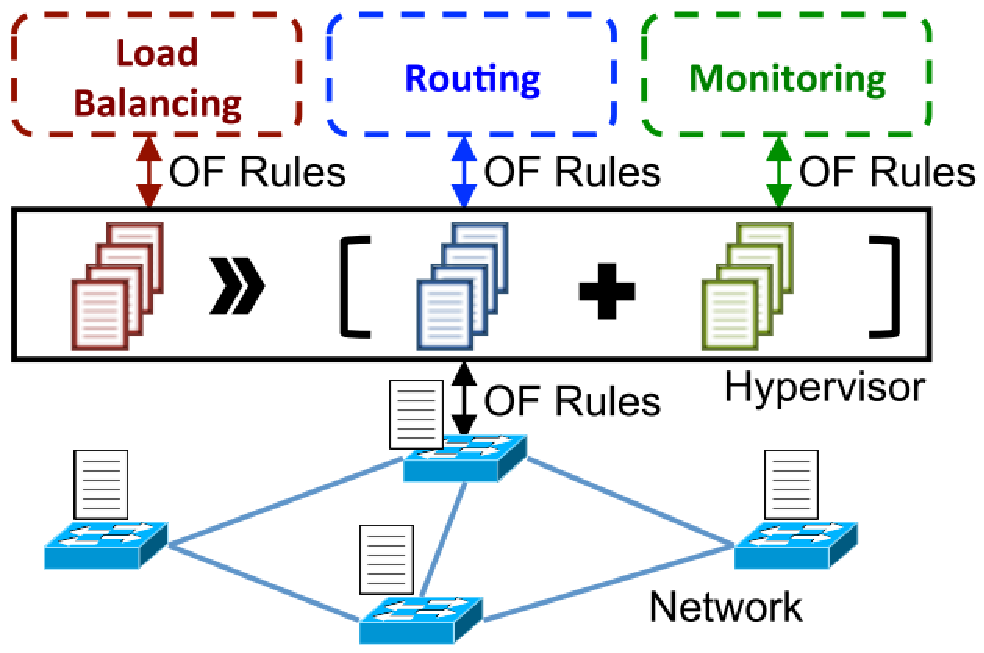
\includegraphics[scale=0.7]{figures/compositional-structure.pdf}
    \caption{Flow rules arithmetic from Compositional Hypervisor~\cite{CompositionalHypervisor-Jin2014}}
    \label{fig:compositional-hyp}
\end{figure}


\subsection{Mapping based hypervisors without migration}
The hypervisors presented in this section maintain a mapping between the Virtual Network they present to the tenant and the physical resources used to embed it but do not support the migration of Virtual Networks.

\subsubsection{ADVisor}
ADVisor~\cite{ADVisor-Salvadori2012} is based on FlowVisor and tackles two design issues introduced by FlowVisor.
The first contribution is the implementation of arbitrary virtual topologies.
Instead of slicing physical resources and presenting them to the tenants, 
The virtualization completely decouples the abstract view of the Virtual Network from the physical resources embedding it.
A virtual link between two virtual nodes might in fact be composed of several physical links. The role of ADVisor is to hide these intermediate nodes from the tenant.

The second contribution of ADVisor consists in sharing the flowspace proposed by FlowVisor.
Originally, the definition of a flowspace would restrict the manipulation of a certain type of traffic (\eg port 80, filter by source MAC address) to only one tenant.
Giving access of one flowspace to two different tenants would break the isolation and allow one to control and alter the traffic of the other.
The same limitations hold regarding the address space available to tenants.
ADVisor alleviates this limitation by defining a set of identifiers that will be allocated to each tenant. Each tenant can deploy his OF rules without being limited by the other tenants' configurations, \ie each tenant has access to the whole flowspace (as defined in Section~\ref{def:netvirt}), with the exception of the few bits reserved by ADVisor to store these necessary identifiers.
ADVisor proposes three possible fields to store tenants' identifiers, namely VLAN ID, MPLS labels or 802.1ad multiple VLAN tagging.

\begin{figure}[ht]
    \centering
    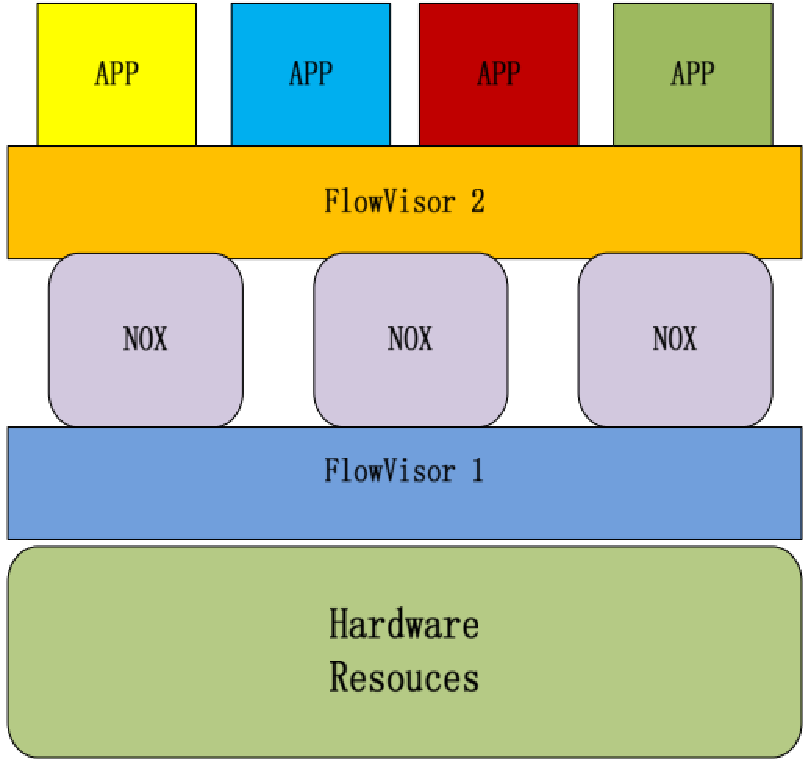
\includegraphics[scale=0.6]{figures/double_fv.pdf}
    \caption{Architecture of Double FlowVisor~\cite{DoubleFV-Yin2013}}
    \label{fig:double-fv}
\end{figure}

\subsubsection{Double FlowVisor}
Double FlowVisor~\cite{DoubleFV-Yin2013} combines two instances of FlowVisor to virtualize a multi-domain network and provide a unified view of the Virtual Network, as presented in Figure~\ref{fig:double-fv}. The first instance of FlowVisor (FlowVisor 1) is used to hide the heterogeneity of the different network domains. These domains are connected together, composing the physical infrastructure, and a NOX controller~\cite{nox-gude2008} is connected to FlowVisor\GB{in the Figure, NOX is linking both FlowVisor layers. Please rewrite the pararaph to highlight the position of NOX.}.
Then, the second FlowVisor instance (FlowVisor 2) connects NOX with the tenants' applications. This instance maintains the embedding between virtual resources and the physical substrate, and translates commands sent by the tenant into commands deployed on the physical infrastructure. In addition to that, the second FlowVisor instance is in charge of tagging each flow with an identifier related to the tenant.

\begin{figure}[ht]
    \centering
    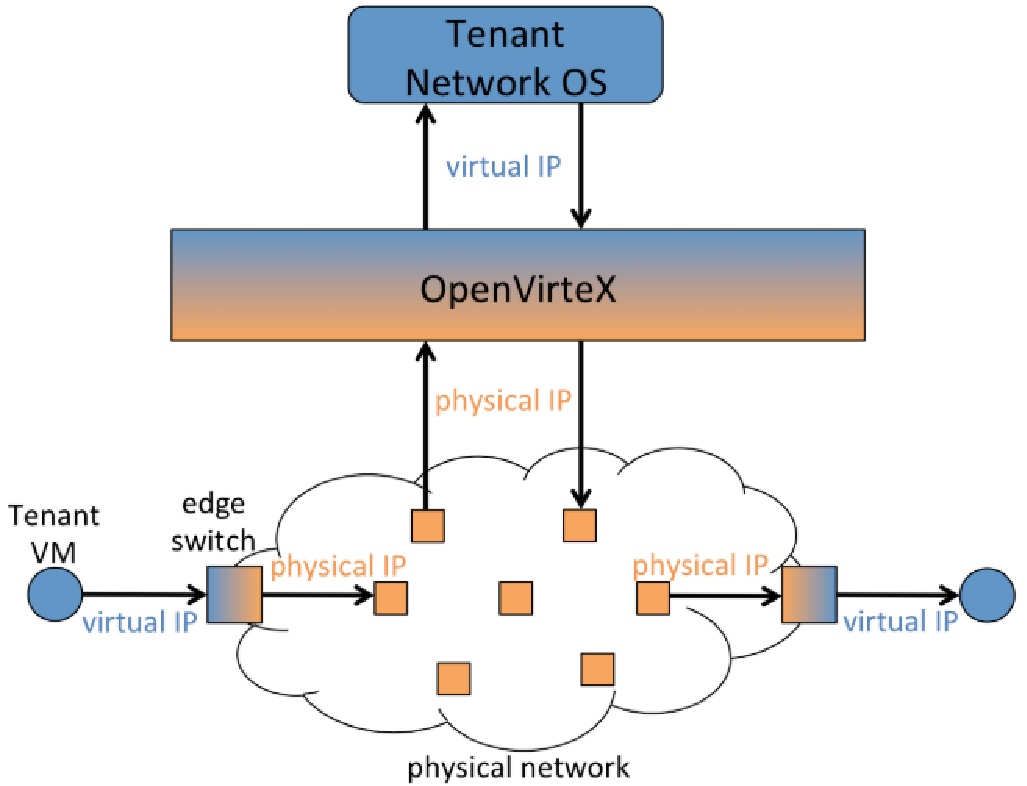
\includegraphics[scale=0.7]{figures/openvirtex.pdf}
    \caption{Identifier translation at edge switches in OpenVirteX~\cite{OpenVirteX-Al-Shabibi2014}}
    \label{fig:openvirtex}
\end{figure}

\subsubsection{OpenVirteX}
OpenVirteX~\cite{OpenVirteX-Al-Shabibi2014} (OVX) is a network hypervisor based on the same design as FlowVisor~\cite{FlowVisor-Sherwood2009}, \ie OVX serves as a proxy between the tenants' controllers and the underlying physical infrastructure. OVX provides both full virtual topology abstraction and full address space abstraction. 

When a tenant requests a Virtual Network, he describes the different resources, nodes and links he needs.
Then OVX will determine the adequate physical substrate to embed the Virtual Network.
The virtual/physical resources mapping is stored by OVX and is used to present the Virtual Network to the controller.
While FlowVisor will hide messages to unintended recipients, OVX intercepts LLDP packets used for topology discovery. Everytime an LLDP message arrives at a virtual switch, OVX uses the mapping to determine the virtual node at the other end of the virtual link. An LLDP response is forged by OVX with matching information and forwarded to the corresponding tenant's controller.

OVX enables tenants to use the full address space by assigning an identifier, stored in the IP and MAC address fields, to each tenant and then combining it with a unique identifier for each host. Figure~\ref{fig:openvirtex} depicts the two cases where the identifier translation is performed. In the first case, when the tenant Network Operating System wants to deploy flow rules, he will specify its own virtual identifiers. OpenVirteX will intercept the flow rules, translate the virtual IP addresses into the corresponding physical ones. The second case is when traffic goes through an edge switch of the physical network, the switch is in charge of translating the IP headers back into the flowspace used by the Virtual Machine (VM).

\subsubsection{SR-PVX}
SR-PVX~\cite{PVX-Li2017} is the first network hypervisor supporting Protocol Oblivious Forwarding~\cite{pof-song2013} (POF). POF is an extension of the concept set up by OpenFlow~\cite{Openflow-McKeown2008}, where developers may implement new protocols without by the design\GB{this is an obvious typo. Please rewrite.} of the OpenFlow protocol (\eg how messages should be formatted and processed).
SR-PVX provides two main features, namely the improved programmability of the POF paradigm and a reduced resource consumption to implement network virtualization.

The programmability proposed by POF consists in replacing protocol specific headers by a set of \textit{\{offset,length\}} tuples. This way, developers will be able to specify their own data structures and how the switch will process them, instead of being constrained by existing structures, like Ethernet and IP headers for instance. This allows to encapsulate tenants identifiers on top of the packet, and to  use Source Routing (SR), where routing instructions are also encapsulated inside the packet to route it across the network instead of being stored in each switch.
Upon receiving a Virtual Network request, a Network Embedder will determine the optimal physical substrate. Then the hypervisor will generate the related specific forwarding instructions and deploy them only on the physical switches used to embed virtual nodes. Every other physical switch used to connect two virtual nodes is hidden from the tenant's view and is abstracted as part of the virtual link.

In SR-PVX, the authors outline the physical limitations encountered by physical switches.
Traditional network hypervisors quickly reach the maximum capacities of the network equipments because of the high number of users and the regular changes in the infrastructure due to failures or VM relocation. The SR paradigm is leveraged to tackle this issue. Each physical node embedding a virtual node stores encapsulation rules toward the next virtual node. Between them may sit several switches with no rules deployed. Instead, they treat incoming traffic by decapsulating the next available header indicating which port the packet must be sent to. By reducing the number of switches on which the rules must be installed, SR-PVX greatly improves the resource consumption of SDN virtualization. The authors propose in~\cite{pvflow-Li2018} a flowtable virtualization mechanism that improves the work done with the design of SR-PVX by reducing the number of flow rules required for each tenant.
    

\subsubsection{WhiteVisor}
WhiteVisor~\cite{whitevisor-Yu2019} is designed to support SDN-based virtualization on white box switches (\ie bare metal equipments).
White box switches are networking elements that do not natively embark any operating system and simply provide network forwarding functions that will be used by the operating system.  
The main challenge of using these switches is that they provide a specific set of instructions and flow tables to process packets. 
WhiteVisor uses the VLAN ID field to identify tenants.
Moreover, the L2 and L3 routing is not performed on the same flow tables and associated pipelines.
WhiteVisor is based on two main components, a virtual to physical pipeline converter as well as a storage component.
A pipeline is a sequence of processing functions used for a specific flow.
The pipeline converter translates a virtual pipeline by taking each processing function, translating the virtual identifiers into physical ones and generating the corresponding flow rules. These rules are then installed in the different flow tables of the white box switches. WhiteVisor implements both Layer 2 and Layer 3 routing and details the different mechanisms associated to each routing scheme. The authors also highlight the technical constraints of white box switching related to the ordering of flow processing and header matching. The storage component is used to keep a mapping of the physical and virtual pipelines and to notify tenants when a pipeline is removed. 


\subsubsection{ONVisor}
ONVisor~\cite{ONVisor-Han2018} is a network hypervisor based on the ONOS~\cite{onos-Berde2014a} controller.
It has been designed along three main ideas: a distributed hypervisor to provide flexibility and scalability, an abstraction of the heterogeneous hardware and protocols implementations (\eg various implementations of OpenFlow v1.3),  and finally, VN federation to allow different Virtual Networks of a same tenant to interact.
ONVisor implements network virtualization by extending ONOS's SouthBound Interface.
Precisely, ONVisor implements two new components, the \textit{Virtual Provider} and the \textit{Virtual Manager}.
The \textit{Virtual Manager} provides tenants with service interfaces, similarly to the northbound interface implemented by ONOS. 
Tenants are identified by using an identifier encapsulated in the packets.
Tenants are able to interact with their VN through this component.
The \textit{Virtual Provider} in turn receives the commands sent from the \textit{Virtual Manager} and translates them so they can be deployed in the physical infrastructure. This component also receives networking events and translates them before forwarding them to the tenants' applications.

\subsection{Mapping based hypervisors supporting the migration}
The hypervisors presented in this section abstract the physical resources behind a mapping with the Virtual Network presented to the tenant. In opposition to the previous section, these hypervisors provide a form of Virtual Network migration. 

\subsubsection{VeRTIGO}
VeRTIGO~\cite{VeRTIGO-Corin2012a} is an extension of the work done with ADVisor and offers two different types of Virtual Networks.
Either the tenant has the full control over the Virtual Network (including traffic engineering techniques) or he is presented with a single node and leave the handling of network operations to the service provider.
The latter abstract view is often referred to as the ``Big Switch Abstraction".
It provides a Virtual Network to a tenant who is not interested in handling network operations himself.
VeRTIGO identifies tenants by storing the header sequence of each flow in a database.

VeRTIGO implements Virtual Network migration using a component called VT Planner. The VT Planner consists in a set of precached virtual topologies that is deployed in case of a link failure. In case of a link congestion or a physical failure, the VT Planner migrates the Virtual Network by deploying the configuration rules into the corresponding network equipments.

\subsubsection{CoVisor}
CoVisor~\cite{CoVisor-Jin2015} extends Compositional Hypervisor~\cite{CompositionalHypervisor-Jin2014} by making two significant contributions.
The first one is a novel policy combination algorithm that focuses on the performance of the policy deployment in terms of packets sent and computation time.
CoVisor exploits the policies being composed to generate specific data structures that will serve as rule identifiers.
Regrouping composed policies based on the common fields they affect reduces the number of rules  considered at compilation time.
Similarly, they correlate common attributes between policies to serve as identifiers for storage. The intersection of the matching fields for two policies determines the identifier storage for the composed policy.
This algorithm also supports the case where a single physical node spans multiple virtual switches.

The second contribution is related to the view provided by the hypervisor to each application.
CoVisor presents an abstract view of the topology based on the operational needs of the application, thus enhancing the security of the infrastructure by only granting rights for the requested usage. 
For instance, a firewall may only see the infrastructure as a big switch since the incoming traffic should be dropped at the ingress point of the network.
Similarly, a routing application will require full access to the network to determine the optimal routing paths.
CoVisor also limits the actions available to each application using a fine-grained control over the capacities of each controller.
For example, a MAC learner application should only match packets based on MAC addresses, or a firewall should only be able to accept or drop packets, and not to modify them.
By design, CoVisor implements two fail-over mechanisms regarding controller failures and switch failures.
Controller failure is handled by introducing a third operator in the policy composition, namely the override operator. The first two operators introduced by Compositional Hypervisor are the sequential and parallel policy composition operators. The override operator specifies which policy to apply if every other fails.
In case of a physical failure of a switch, CoVisor notifies each application impacted by the failure and redeploys required OF rules elsewhere in the network when possible.


\subsubsection{FlowN}
FlowN~\cite{FlowN-Drutskoy2012} is a network hypervisor designed to provide a full abstraction of the physical infrastructure and to propose a container-based application virtualization system. 
The hypervisor serves each tenant with a custom virtual topology. The virtual topology requires a specific number of nodes and links but FlowN also implements bandwidth reservation as well as maximum latency per link. 
In case of a switch or link failure, FlowN will migrate the virtual node on a new physical switch without notifying the impacted tenants.

% The virtualization of the control layer places FlowN between tenants' applications and the physical infrastructure\GB{as usual}. 
When an SDN application makes a function call, FlowN intercepts it and translates it to preserve the mapping between the virtual address space and the physical address space. Since FlowN is based on the NOX~\cite{nox-gude2008} SDN controller, tenants application are limited by the capacities of this controller. 
% The design of an API between applications and the hypervisor is in opposition to the concept of FlowVisor~\cite{FlowVisor-Sherwood2009} where tenants directly interact with the physical nodes and FlowVisor only restrict and translate OF rules to respect the isolation requirements of the virtualization.

FlowN also offers the full abstraction of the address space for the tenants.
Each tenant is able to use all the header fields, and FlowN maintains the mapping between the physical node address space and the virtual one inside a database. FlowN uses encapsulation at the ingress point to determine to which tenant the packet must be forwarded to. Encapsulation is based on VLAN tagging, in a fashion similar to Nicira~\cite{nicira}\GB{Nicira is a brand. You are referring to the Network Virtualization Platform.}.   
FlowN leverages databases to simplify the mapping of physical and virtual elements, and to add consistency in the network state view.  


\subsubsection{AutoSlice}
AutoSlice~\cite{AutoSlice-Bozakov2012} is designed to tackle the scalability issues of a distributed hypervisor, and optimize the resource consumption of physical switches to overcome specific limitations.
In~\cite{AutoSlice-Bozakov2012}, the authors present the basis of the AutoSlice hypervisor.
Each physical SDN infrastructure is managed by its own controller proxy (CPX).
Each CPX is in charge of accessing corresponding physical switches and translating OF rules from the virtual flowspace to the physical one.
AutoSlice instantiates Virtual Networks over several SDN domains and each CPX deploys the corresponding OF rules in their infrastructure.
Each CPX is in charge of migrating virtual resources within their own domain.
AutoSlice overcomes the physical limitations of Openflow switches by delegating part of OF rules storage to a set of software switches.
These switches are running on commodity servers and therefore have the sufficient resources to store all the possible OF rules.
AutoSlice uses a statistical distribution to assume that low volume flows will generate most of the OF rules and store them in the software switches. In opposition, the biggest volume flows use a rather small set of OF rules and deploy them inside the physical switches.
In~\cite{AutoSlice2-Bozakov2014}, the authors go into more details about several design requirements they have expressed. They extend the notion of isolation between tenants by introducing a set of identifiers to prevent the overlap of OpenFlow rules installed by different tenants.
The isolation of flow tables is ensured by adding a \textit{Virtual Table Identifier}, thus sharing the physical flow table among the different tenants.
Similarly, all packets are tagged with a \textit{Packet Identifier} so it can be mapped with the \textit{Virtual Table Identifier} and determine the tenant and how the packet should be processed.
The authors also propose Virtual Network migration techniques based on information duplication, and highlight the potential excessive usage of flow table resources.
% There is no evaluation provided in both~\cite{AutoSlice-Bozakov2012} and~\cite{AutoSlice2-Bozakov2014}.

\subsubsection{NVP}
The Network Virtualization Platform~\cite{NVP-Koponen2014} (NVP) proposes a network hypervisor for multi-tenant datacenters. Instead of focusing on virtualizing the physical network of the data center, NVP provides a Virtual Network on top of the OpenvSwitches~\cite{openvswitch} deployed in each VMWare Hypervisor. These software switches are then interconnected using tunnels for end-to-end communication. 
The physical network is simply used to support these tunnels and is assumed to possess standard capacities.
The paper makes several contributions: the implementation of logical networks based on OpenvSwitch (OVS), the creation of a Domain Specific Language (DSL) to declare the connectivity between hypervisors, switches and more generally the forwarding rules of all network equipments.
% \etc and tackle scalability and availability issues encountered by NVP.

The logical networks proposed to a tenant in NVP consist in creating a fully meshed Virtual Network between every compute node running the tenant's VMs.
The creation of the Virtual Network is as follows:
each VM hypervisor hosting VMs belonging to a tenant will instantiate a \textit{logical datapath}\GB{please briefly explain what a datapath is since it is first mentioned here} inside its own OVS. 
Then, for each pair of logical datapaths that have been created, NVP will create a tunnel between them.
Each time an incoming packet goes through an ingress port of the hypervisor, the packet will be redirected to the correct\GB{what does ``correct'' mean here?} logical datapath then transmitted to the logical datapath corresponding to the destination VM.
The tenant can configure these datapaths with regard to switching, routing and security matters, similarly to legacy networking elements.
The isolation between tenants is ensured by assigning unique identifiers to each logical datapath, preventing unauthorized access to the tenant's traffic.
NVP implements failover mechanisms of physical networking elements, as well as controllers, by running backup nodes supporting similar functions, which will be used in case of a failure.
A load balancing mechanism is used to replace a failed node by one of the backup nodes.

NVP introduces \textit{nlog}, a DSL proposed to tackle the computational challenge of keeping up with the evolution of the forwarding state inside the logical datapaths. Changes in the forwarding state include arrivals and departures of tenants inside the infrastructure, migration of the different VMs, reconfiguration of logical datapaths by the tenants. \textit{nlog} presents a logical abstraction that decouples the concrete forwarding state and rules from the logic described by NVP. Note that \textit{nlog} is not used by tenants but by NVP when instantiating logical datapaths for tenants.
Tenants are provided an API to interact with NVP.
Using \textit{nlog} to describe the state of the logical abstractions enables an incremental computing of the forwarding state that is resource efficient compared to a naive implementation where any change requires the full recalculation of the forwarding state.

% Scalability inside NVP is ensured by distributing computation over several logical and physical controllers. Logical controllers compute the flow and tunnels corresponding to datapaths. Physical controllers are in charge of the communication with the different service nodes, gateways and hypervisors.
% NVP enforces VN migration in case of a failover of either the physical or logical layer using a sharding mechanism similar to the one used in cluster nodes~\cite{sharding}. 
% A sharding coordinator will monitor the signals sent by the different nodes and will promote a node to the master role if the current master fails.

% The evaluation of NVP focuses on two things, the time and resources required to setup NVP in different scenarios and the available throughput based on which tunneling mechanism is used by NVP. Theses results are then followed by a serie of reflexions based on the experience gained after the implementation of NVP and how design challenges have been tackled.

\begin{figure}[ht]
    \centering
    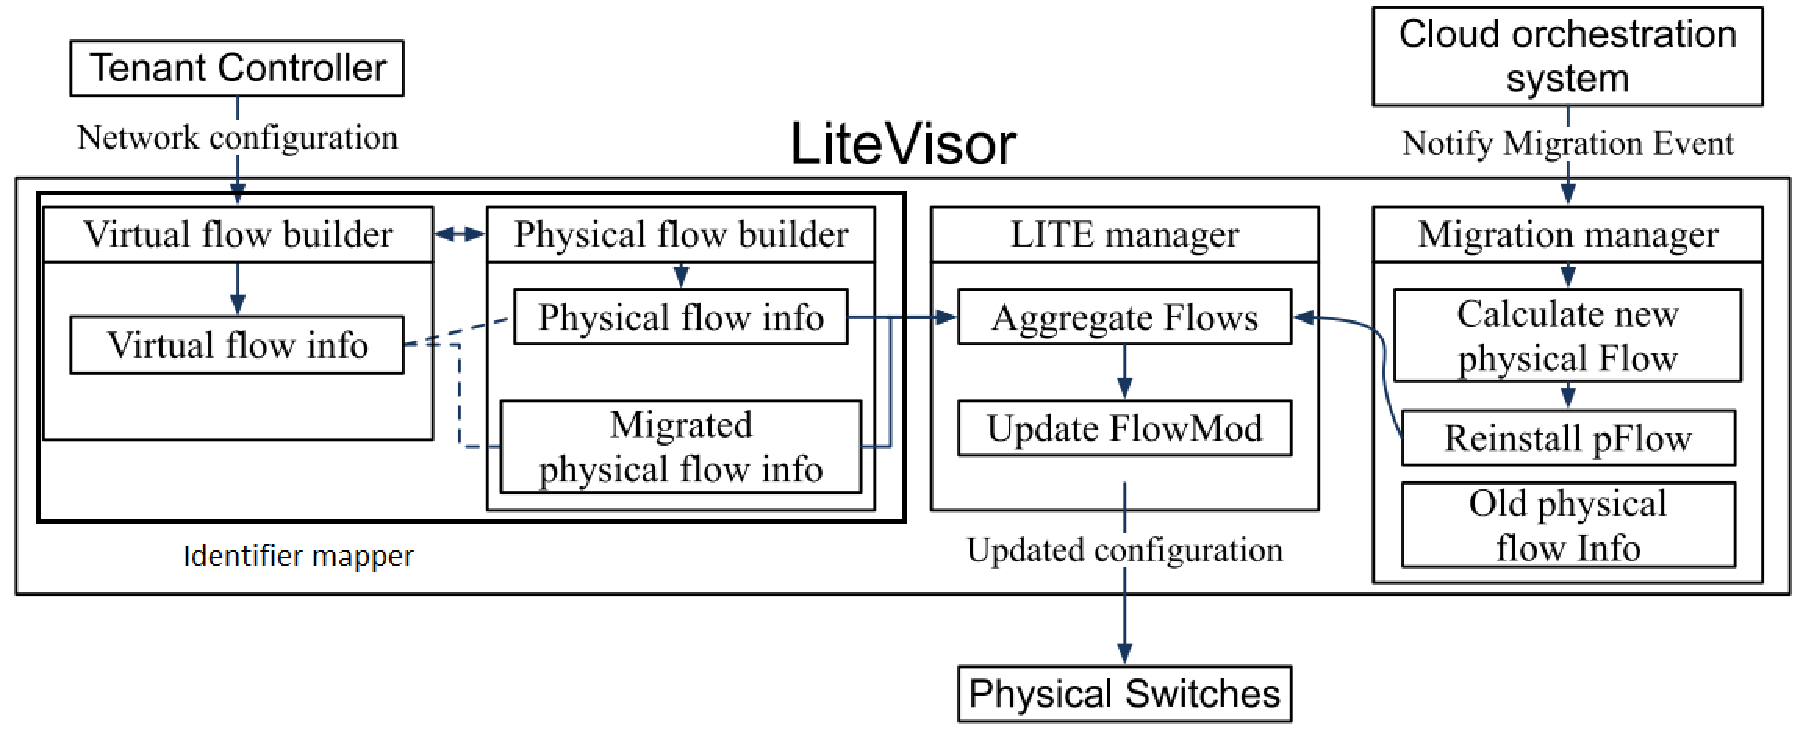
\includegraphics[scale=0.5]{figures/litevisor.pdf}
    \caption{LiteVisor architecture~\cite{Litevisor-Yang2018}}
    \label{fig:litevisor}
\end{figure}

\subsubsection{LiteVisor}
LiteVisor~\cite{Litevisor-Yang2018} is an SDN hypervisor supporting network reconfiguration for VM migration.
The authors outline the previous work on flow aggregation to reduce the consumption of switch resources as well as the performance-sensitive context of datacenters and the limitations of existing encapsulation techniques.
LiteVisor is divided in three components illustrated in Figure~\ref{fig:litevisor}. The identifier mapper translates messages sent between tenants and the hypervisor by rewriting the identifiers inside each message. Identifiers may be stored in either the IP header or the VxLAN ID field.
The second component is the LITE manager, responsible for aggregating flows sent by the tenant's controller, as well as deploying them on the physical switches. 
The last component is the migration manager. When a VM is migrated, the cloud orchestration system notifies the migration manager about the new location of the VM. The manager then computes a new physical flow that will be transmitted to the LITE manager, which in turns decides if it can be aggregated with an existing flow, or deploys it according to configuration rules in the physical infrastructure.




Table~\ref{tab:existing-nhv}\GB{in the reference column, to keep it short, you could either put the author name or the proposal name but not both.} summarizes existing hypervisors, the type of abstraction used to present each tenant with his Virtual Network and whether or not the hypervisor handles the migration of Virtual Networks.
